\documentclass[a4paper,twoside]{article}
\usepackage[T1]{fontenc}
\usepackage[bahasa]{babel}
\usepackage{graphicx}
\usepackage{graphics}
\usepackage{float}
\usepackage[cm]{fullpage}
\pagestyle{myheadings}
\usepackage{etoolbox}
\usepackage{setspace} 
\usepackage{lipsum} 
\graphicspath{ {./images/} }
\setlength{\headsep}{30pt}
\usepackage[inner=2cm,outer=2.5cm,top=2.5cm,bottom=2cm]{geometry} %margin
% \pagestyle{empty}

\makeatletter
\renewcommand{\@maketitle} {\begin{center} {\LARGE \textbf{ \textsc{\@title}} \par} \bigskip {\large \textbf{\textsc{\@author}} }\end{center} }
\renewcommand{\thispagestyle}[1]{}
\markright{\textbf{\textsc{AIF234001 \textemdash Tugas Akhir 1 \textemdash Sem. Ganjil 2023/2024}}}

\newcommand{\HRule}{\rule{\linewidth}{0.4mm}}
\renewcommand{\baselinestretch}{1}
\setlength{\parindent}{0 pt}
\setlength{\parskip}{6 pt}

\onehalfspacing
 
\begin{document}

\title{\@judultopik}
\author{\nama \textendash \@npm} 

%tulis nama dan NPM anda di sini:
\newcommand{\nama}{Nathanael Adi Trianto}
\newcommand{\@npm}{6181901041}
\newcommand{\@judultopik}{Pembuatan Ulang Aplikasi Rugby Indonesia dengan Ionic 7 dan Capacitor} % Judul/topik anda
\newcommand{\jumpemb}{1} % Jumlah pembimbing, 1 atau 2
\newcommand{\tanggal}{22/09/2023}

% Dokumen hasil template ini harus dicetak bolak-balik !!!!

\maketitle

\pagenumbering{arabic}

\section{Deskripsi}
Olahraga adalah aktivitas fisik yang dilakukan untuk menguatkan dan menyehatkan tubuh. Olahraga memiliki berbagai jenis dan tujuan, seperti meningkatkan kesehatan tubuh, meningkatkan daya tahan fisik, meningkatkan kebugaran, dan meningkatkan keterampilan dalam suatu cabang olahraga. Beberapa jenis olahraga yang populer antara lain sepak bola, berenang, tolak peluru, dan permainan bola besar. Olahraga dapat membantu menjaga berat badan ideal, membentuk dan menguatkan otot, baik untuk kesehatan jantung, meningkatkan tinggi badan, dan membuat tubuh rileks. Selain itu, olahraga juga dapat membantu meningkatkan kesehatan mental dan melepaskan tegangan otot atau sendi. Setiap jenis olahraga memiliki teknik dan peraturan yang berbeda-beda, seperti teknik dasar dalam olahraga tolak peluru dan aturan dalam permainan sepak bola.

Rugby adalah salah satu olahraga bola yang dimainkan oleh dua tim. Berdasarkan jumlah pemainnya, olahraga rugby terbagi menjadi 3 jenis utama, yaitu:

\begin{itemize}
    \item Rugby union: setiap tim terdiri dari 15 pemain.
    \item Liga rugby: setiap tim terdiri dari 13 pemain.
    \item Rugby sevens: setiap terdiri dari 7 pemain.
\end{itemize}

Masing-masing tim diharuskan untuk mencetak poin dengan menendang, melempar, membawa dan mendaratkan bola melewati gawang atau garis belakang tim lawan.

Bola yang digunakan pada olahraga rugby memiliki ciri khas, yaitu berbentuk lonjong dan mengerucut pada bagian ujungnya. Dengan bentuknya ini, bola rugby jadi lebih mudah dipegang dan dibawa oleh para pemain selama pertandingan berlangsung.

Sejarah permainan rugby dimulai dari kota Rugby, Inggris pada tahun 1823. Permainan tersebut dicetuskan oleh seorang pemuda bernama William Webb Ellis ketika bermain sepak bola dengan teman-temannya, William mengambil bola dan berlari menuju gawang tim lawan untuk mencetak skor. Seiring berjalannya waktu, rugby terus berkembang dan membentuk federasinya yang pertama, yaitu Rugby Football Union, pada tahun 1871. Keberhasilannya semakin mengukuhkan statusnya ketika rugby pertama kali dipertandingkan secara resmi dalam ajang turnamen olahraga internasional yaitu Olimpiade, pada tahun 1900. Meskipun sempat absen dari Olimpiade pada tahun 1924, rugby kembali sebagai cabang olahraga resmi dalam turnamen Olimpiade tahun 2016 dan tetap relevan hingga saat ini.

Ionic Framework adalah toolkit UI open-source untuk membangun aplikasi modern, cross-platform yang berkualitas tinggi dari satu kode sumber dengan JavaScript dan web. Ionic menyediakan alat dan layanan untuk mengembangkan aplikasi hybrid mobile, desktop, dan progressive web berdasarkan teknologi dan praktik pengembangan web modern, menggunakan teknologi web seperti CSS, HTML5, dan Sass. Ionic 7 adalah versi \textit{stable release} terbaru dari Ionic, yang memperkenalkan cara kerja yang lebih efisien dengan kontrol formulir seperti Toggle atau Input. Komponen Item dan Label tidak lagi diperlukan, dan setiap kontrol formulir menangani konten label secara langsung. Selain itu, fitur tertentu seperti teks bantuan atau mode pengisian input telah dipindahkan dari ion-item ke kontrol formulir yang sesuai seperti ion-input, ion-textarea, dan ion-select. Perubahan ini mengurangi boilerplate kode dengan menghilangkan persyaratan ion-item dan ion-label. Komponen Ionic Framework secara otomatis menyesuaikan tampilan dan nuansa mereka dengan platform di mana mereka berjalan, memungkinkan gestur dan perilaku native yang sama dengan yang biasa digunakan pengguna. Ionic memiliki lebih dari 100 komponen UI yang telah dirancang sebelumnya, tipografi, dan tema dasar yang menyesuaikan dengan setiap platform. Ini dioptimalkan untuk mobile dengan animasi yang diakselerasi oleh hardware, lazy loading, dan scrolling 60FPS. Ionic CLI digunakan untuk membuat, membangun, dan menguji aplikasi serta memanfaatkan Live Reload, deployment, dan dokumen yang sangat baik.

Capacitor adalah runtime native cross-platform yang memudahkan pembuatan aplikasi mobile yang performanya tinggi dan berjalan secara native di iOS, Android, dan platform lainnya menggunakan web tooling modern. Capacitor merupakan evolusi selanjutnya dari aplikasi hybrid, yang menciptakan aplikasi Web Native dengan pendekatan kontainer native modern untuk tim yang ingin membangun aplikasi web-first tanpa mengorbankan akses penuh ke SDK native ketika dibutuhkan. Capacitor menyediakan kumpulan API yang konsisten dan berfokus pada web yang memungkinkan aplikasi tetap dekat dengan standar web sebanyak mungkin, sambil mengakses fitur perangkat native yang kaya pada platform yang mendukungnya. Capacitor dapat menambahkan fungsionalitas native dengan mudah menggunakan Plugin API untuk Swift di iOS, Java di Android, dan JavaScript untuk web. Capacitor 3.0 memiliki peningkatan kinerja, pengalaman untuk mengembangkan yang lebih baik, dan keterlibatan komunitas yang lebih besar. Capacitor dapat diintegrasikan dengan mudah ke dalam proyek JavaScript modern yang ada atau proyek Capacitor yang baru.

Sekitar tahun 2015, perusahaan PT DNArtworks Komunikasi Visual membuat aplikasi Rugby Indonesia yang memanfaatkan Apache Cordova. Aplikasi tersebut memiliki: 
\begin{itemize}
    \item Halaman \textit{Latest News} yang diambil dari https://rugbyindonesia.or.id dengan memanfaatkan protokol RSS.
    \item Halaman \textbf{Fixture \& Results} yang diambil dari https://rugbyindonesia.or.id.
    \item Halaman \textit{Teammate Photos} dengan fungsi:
    \begin{itemize}
        \item Pengguna dapat langsung mengambil foto dari aplikasi tersebut.
        \item Pengguna dapat langsung memberikan frame terhadap foto tersebut.
        \item Pengguna dapat langsung menggunggah foto tersebut ke dalam galeri publik.
    \end{itemize}
    \item Halaman \textit{Rugby Clubs} dengan fungsi pengguna dapat langsung mendaftar ke dalam klub rugbi di Indonesia.
    \item Fungsi \textit{Push Notifications}.
\end{itemize}

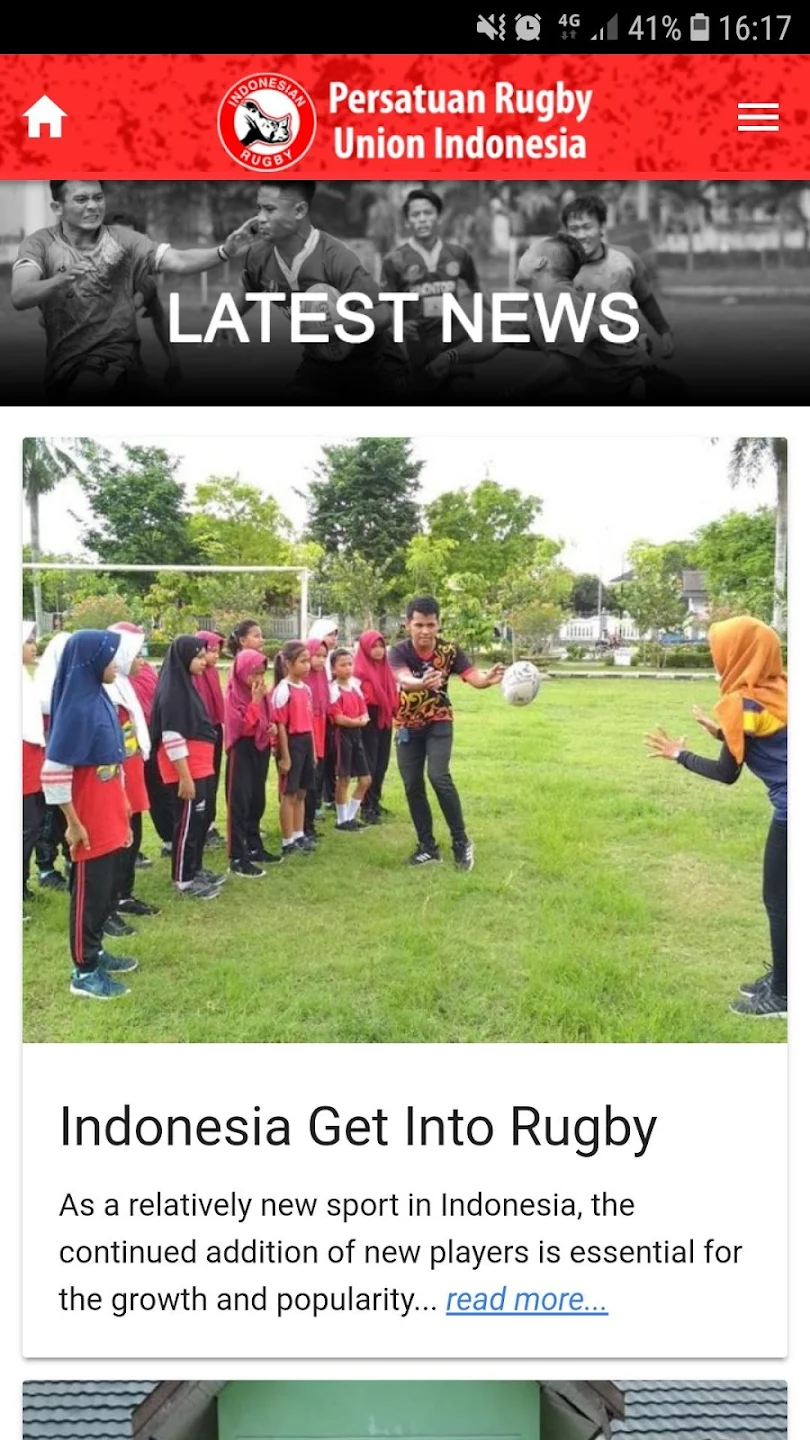
\includegraphics[scale=0.2]{latest_news.png} \hspace{1cm} 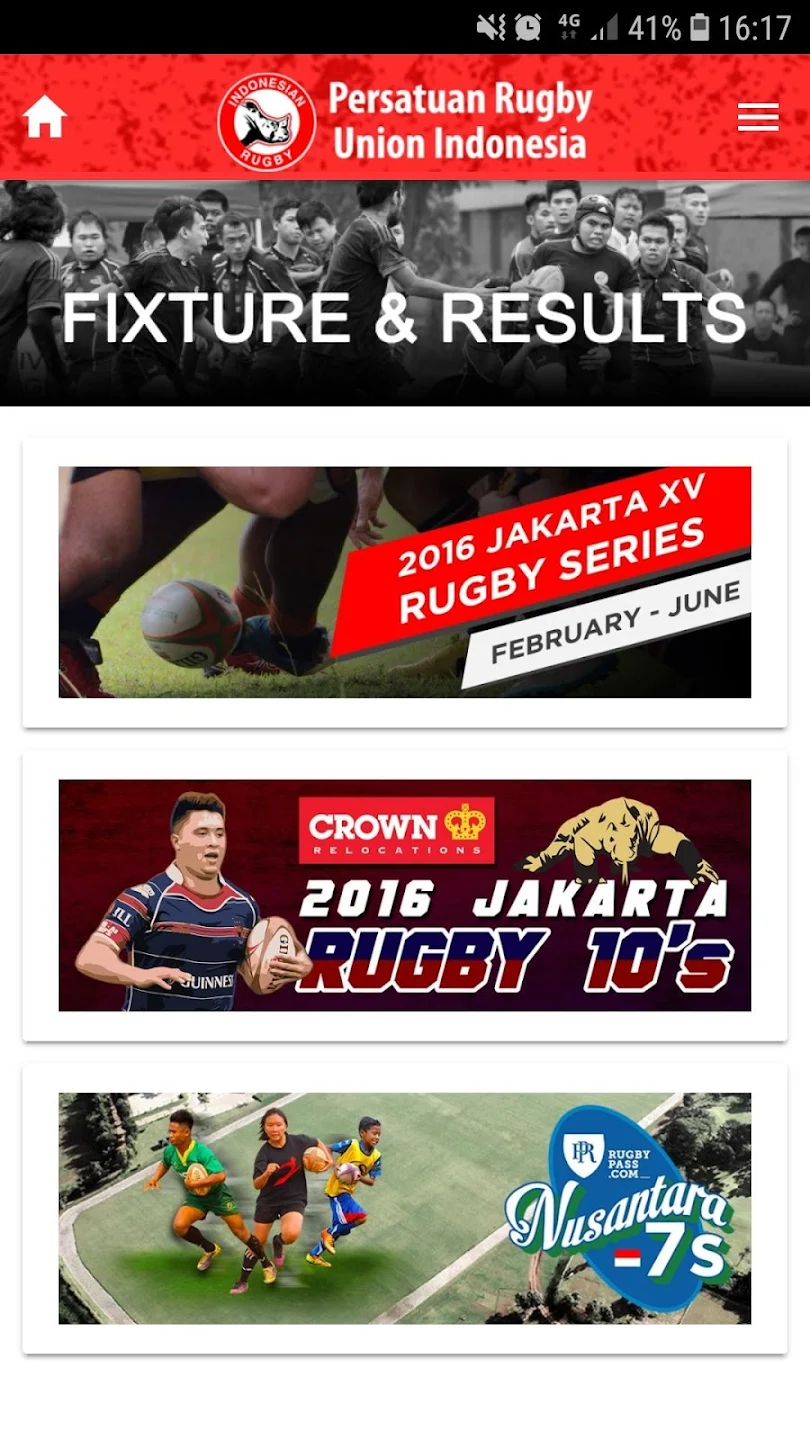
\includegraphics[scale=0.2]{fixture_results.png}

Gambar 1. Halaman Latest News \hspace{1.5cm} Gambar 2. Halaman Fixture \& Results

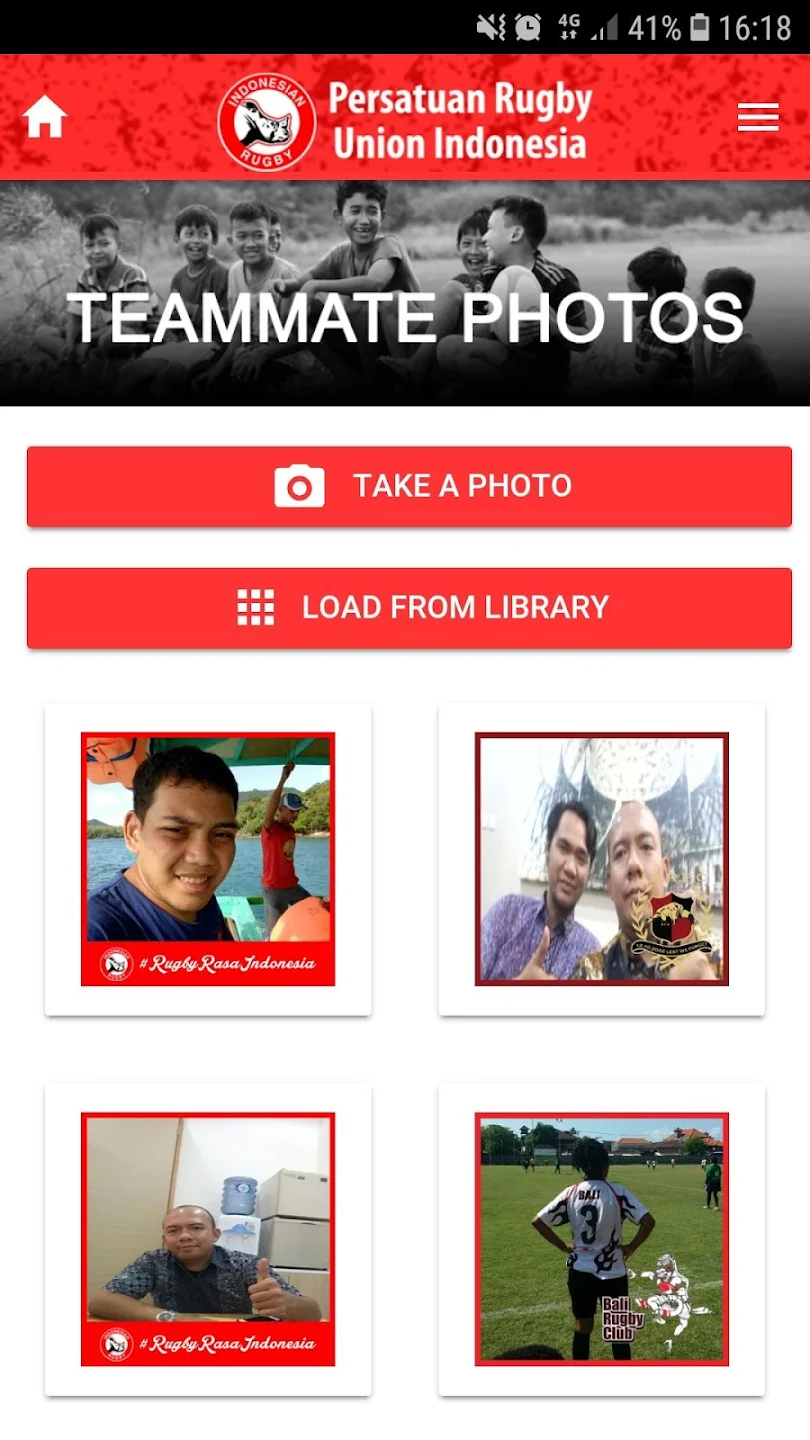
\includegraphics[scale=0.2]{teammate_photos.png} \hspace{1cm} 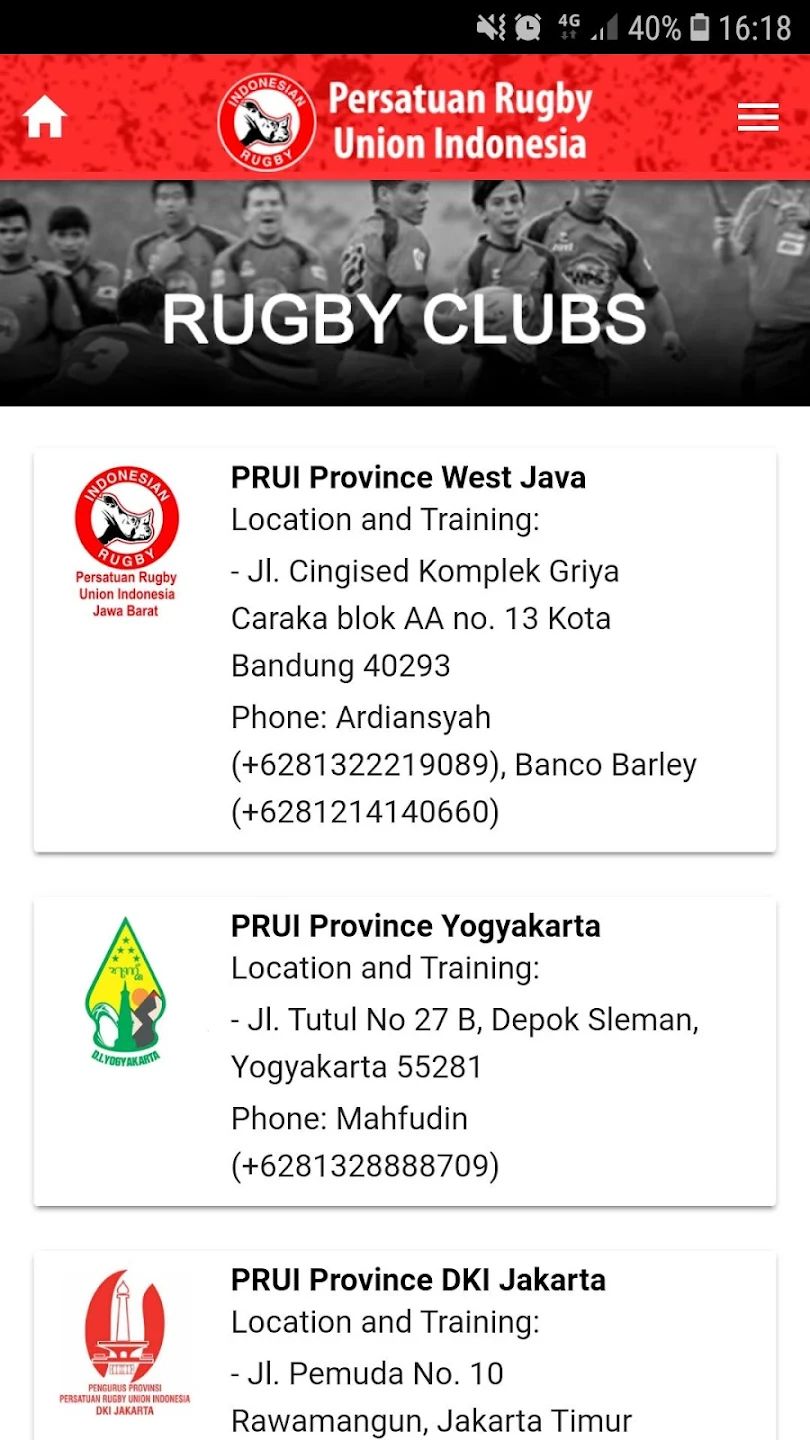
\includegraphics[scale=0.2]{rugby_clubs.png}

Gambar 3. Halaman Teammate Photos \hspace{1cm}  Gambar 4. Halaman Rugby Clubs

% Tuliskan deskripsi dari topik skripsi yang akan anda ajukan. Di sini dapat dituliskan latar belakang, seperti apa penelitian yang sudah ada sebelumnya dan apa yang akan anda kerjakan. Sertakan gambar agar penjelasan anda menjadi lebih baik.

Pada saat ini, aplikasi tersebut masih tersedia di Google Play Store, namun aplikasi tersebut tidak dapat dipasang pada perangkat \textit{android} saat ini dikarenakan website https://rugbyindonesia.or.id sudah berubah dan juga framework yang digunakan sudah terlalu lama. Maka dari itu pada skripsi ini, akan dibuat ulang sebuah perangkat lunak Rugby Indonesia yang terbaru, sehingga perangkat lunak tersebut dapat \textit{compatible} dengan perangkat \textit{android} saat ini.

% Pada skripsi ini, akan dibuat sebuah perangkat lunak yang dapat menampilkan visualisasi dan simulasi kerumunan orang yang berkunjung ke sebuah museum. Dengan menggunakan perangkat lunak tersebut, pengelola museum dapat mengatur tempat peletakan objek sehingga tidak terjadi kerumunan yang terlalu padat.

% Dari berbagai macam teknik yang dapat digunakan untuk melakukan simulasi kerumunan, dipilih dua buah teknik yaitu teknik {\it flow tiles} dan {\it social force model (steering behaviour)}.

% Dst, dst, dst, \ldots\ldots\ldots 

Perangkat lunak ini akan dibuat dengan memanfaatkan bantuan {\it framework} Ionic 7 dan Capacitor dengan:

\begin{itemize}
    \item Halaman \textit{Latest News}, di mana pengguna dapat melihat berita terbaru seputar Rugby Indonesia.
    \item Halaman \textit{Teammate Photos}.
\end{itemize}

% Dst, dst, dst, \ldots\ldots\ldots 

\section{Rumusan Masalah}
Rumusan masalah yang akan dibahas pada skripsi ini adalah sebagai berikut:
\begin{itemize}
    \item   Bagaimana Ionic Framework membantu dalam pengembangan aplikasi mobile, dan apa keunggulan yang ditawarkan oleh Ionic 7?
    \item Bagaimana Capacitor memungkinkan pengembangan aplikasi mobile yang berkinerja tinggi dan berjalan secara native di berbagai platform, dan mengapa menjadi pilihan yang tepat untuk pengembangan ulang aplikasi Rugby Indonesia?
\end{itemize}
% Tuliskan rumusan dari masalah yang akan anda bahas pada skripsi ini. Rumusan masalah biasanya berupa kalimat pertanyaan. Gunakan itemize seperti contoh di bagian Deskripsi Perangkat Lunak.

\section{Tujuan}
Tujuan yang ingin dicapai pada penulisan skripsi ini yaitu:
\begin{itemize}
    \item Menganalisis bagaimana Capacitor memungkinkan pengembangan aplikasi mobile yang berkinerja tinggi dan berjalan secara native di berbagai platform.
    \item Mengidentifikasi alasan-alasan konkret mengapa Capacitor dianggap sebagai pilihan yang tepat untuk pengembangan ulang aplikasi Rugby Indonesia, termasuk aspek-aspek teknis, performa, fleksibilitas, kelebihan, dan kekurangannya.
\end{itemize}

% Tuliskan tujuan dari topik skripsi yang anda ajukan. Tujuan penelitian biasanya berkaitan erat dengan pertanyaan yang diajukan di bagian rumusan masalah. Gunakan itemize seperti contoh di bagian Deskripsi Perangkat Lunak.

\section{Deskripsi Perangkat Lunak}
% Tuliskan deksripsi dari perangkat lunak yang akan anda hasilkan. Apa saja fitur yang disediakan oleh PL tersebut dan apa saja kemampuan dari PL tersebut. Perhatikan contoh di bawah ini:

Perangkat lunak akhir yang akan dibuat memiliki fitur minimal sebagai berikut:
\begin{itemize}
    \item Pengguna dapat melihat berita terbaru yang terdapat pada Rugby Indonesia.
    \item Pengguna dapat melihat foto yang diunggah oleh pengguna tersebut maupun pengunggah lain pada aplikasi Rugby Indonesia.
    \item Pengguna dapat megunduh foto yang terdapat pada aplikasi Rugby Indonesia.
    \item Pengguna dapat mengubah ataupun menghapus unggahan foto pengguna tersebut pada aplikasi Rugby Indonesia, namun tidak dapat melakukan hal tersebut pada foto yang diunggah oleh orang lain.
\end{itemize}

\section{Detail Pengerjaan Skripsi}
Tuliskan bagian-bagian pengerjaan skripsi secara detail. Bagian pekerjaan tersebut mencakup awal hingga akhir skripsi, termasuk di dalamnya pengerjaan dokumentasi skripsi, pengujian, survei, dll.

Bagian-bagian pekerjaan skripsi ini adalah sebagai berikut :
\begin{enumerate}
    \item Mendalami ReactJS sebagai salah satu perpustakaan JavaScript.
    \item Menganalisis aplikasi Rugby Indonesia yang sudah dibuat dengan memanfaatkan Apache Cordova.
    \item Menganalisis fitur-fitur yang dibutuhkan untuk alikasi Rugby Indonesia.
    \item Membuat aplikasi Rugby Indonesia yang sudah memanfaatkan framework Ionic 7 dan juga Capacitor.
    \item Melakukan pengujian dan eksperimen.
    \item Menulis dokumen skripsi
\end{enumerate}

\section{Rencana Kerja}
Rincian capaian yang direncanakan di Skripsi 1 adalah sebagai berikut:
\begin{enumerate}
    \item Mempelajarai, memahami, serta mendalami ReactJS sebagai salah satu perpustakaan JavaScript yang akan digunakan pada skripsi ini.
    \item Mempelajari, memahami, dan mendalami framework Ionic 7 serta Capacitor.
    \item Menganalisis kebutuhan fitur yang diperlukan untuk aplikasi Rugby Indonesia.
    \item Menulis dokumen skripsi dari Bab 1 hingga Bab 3.
\end{enumerate}

Sedangkan yang akan diselesaikan di Skripsi 2 adalah sebagai berikut:
\begin{enumerate}
    \item Membuat aplikasi Rugby Indonesia yang sudah memanfaatkan framework Ionic 7 serta Capacitor.
    \item Melakukan pengujian dan juga eksperimen terhadap aplikasi yang akan dibuat.
    \item Menulis dokumen skripsi dari Bab 4 hingga selesai.
\end{enumerate}

\vspace{1cm}
\centering Bandung, \tanggal\\
\vspace{2cm} \nama \\ 
\vspace{1cm}

Menyetujui, \\
\ifdefstring{\jumpemb}{2}{
\vspace{1.5cm}
\begin{centering} Menyetujui,\\ \end{centering} \vspace{0.75cm}
\begin{minipage}[b]{0.45\linewidth}
% \centering Bandung, \makebox[0.5cm]{\hrulefill}/\makebox[0.5cm]{\hrulefill}/2013 \\
\vspace{2cm} Nama: \makebox[3cm]{\hrulefill}\\ Pembimbing Utama
\end{minipage} \hspace{0.5cm}
\begin{minipage}[b]{0.45\linewidth}
% \centering Bandung, \makebox[0.5cm]{\hrulefill}/\makebox[0.5cm]{\hrulefill}/2013\\
\vspace{2cm} Nama: \makebox[3cm]{\hrulefill}\\ Pembimbing Pendamping
\end{minipage}
\vspace{0.5cm}
}{
% \centering Bandung, \makebox[0.5cm]{\hrulefill}/\makebox[0.5cm]{\hrulefill}/2013\\
\vspace{2cm} Pascal Alfadian Nugroho, S.Kom., M.Comp.
}
\end{document}

